% Use style package recommended by conference.
\documentclass[letterpaper,single,9pt]{article}

\usepackage[all=normal, paragraphs, indent, lists, floats, sections, title]{savetrees}

\usepackage{epsfig}
\usepackage{graphicx}
%\usepackage{subfigure}
\usepackage{subcaption}
\usepackage{verbatim}
\usepackage{amsmath,amssymb}
\usepackage{color}
\usepackage[hyphens]{url}
\usepackage{listings}
\usepackage[normalem]{ulem}
\usepackage{floatrow}
\usepackage{xspace}
\usepackage{amsmath}
\usepackage{enumitem}
\usepackage{booktabs}
\usepackage[utf8]{inputenc}
\usepackage{authblk}
\usepackage{hyperref}
\usepackage{algorithm, algpseudocode}
\usepackage{fancyvrb}
\usepackage{cprotect}
\usepackage{mdframed}
\usepackage{array}
\usepackage{cite}
\usepackage{multirow}
\usepackage{caption}
\usepackage{listings}
\usepackage[usenames,dvipsnames]{xcolor}
\newcommand\independent{\protect\mathpalette{\protect\independenT}{\perp}}
\def\independenT#1#2{\mathrel{\rlap{$#1#2$}\mkern2mu{#1#2}}}
%\renewcommand{\theenumi}{\Alph{enumi}}
\begin{document}
\title{COMS W4771 - Machine Learning 5th Exersice}

  \author{ {\rm Georgios Koloventzos - gk2409} \\ }

\maketitle

\section*{1}
The problem described here is the famous Monty hall problem.
We will analyze the what happens when you choose the first door as
your choise. W.l.o.g. is the same if you choose any of the other 2 doors.
Let assume that the C$x$ event is that the car is behind door $x$.
So $P(Cx) = \frac{1}{3}$. Also let assume that user choosing door $x$ is D$x$.
Also host opening door $x$ is represented H$x$. Also $P(Cx\mid D1) = \frac{1}{3}$.
Also we have the probabilities:
\begin{align*}
P(H3\mid C1,D1) &= \frac{1}{2}\\
P(H3\mid C2,D1) &= 1\\
P(H3\mid C3,D1) &= 0
\end{align*}
Because if the car is in behind door 1 then the host can open any of the other 2.
If car is behind door 2 then he has to open the 3rd door. And it will not open the 
3rd door if the car is behind that door. So if the player select door 1 and the host
opens the 3rd, the probability of winning by switching is:
\begin{align*}
P(C2\mid H3,D1) &= \frac{P(H3\mid C2,D1) P(C2\mid D1)}{P(H3\mid D1)}\\
&= \frac{P(H3\mid C2,D1) P(C2\mid D1)}{P(H3\mid C1,D1) P(C1\mid X1) + P(H3\mid C2,D1) P(C2\mid X1) + P(H3\mid C3,D1) P(C3\mid X1)}\\
&= \frac{P(H3\mid C2,D1)}{P(H3\mid C1,D1) + P(H3\mid C2,D1) + P(H3\mid C3,D1)}\\
&= \frac{1}{\frac{1}{2} + 1 + 0} = \frac{2}{3}
\end{align*}
So it is better to change doors.

\section*{2}
The propability $p(x_1,\dotsc,x_5) = \prod_{i=i}^5 p(x_i\mid \pi_i)$.
So for our graph we have:
\begin{align*}
p(x_1,\dotsc,x_5) = p(x_1)p(x_3)p(x_2\mid x_1)p(x_4\mid x_{1},x_3)p(x_5\mid x_{2},x_4)
\end{align*}
\begin{enumerate}
\item False. As no node is shaded the ball can go from $x_2$ to $x_1$ and reach $x_4$ (2 effects handout 15 p.12)
\item False. As $x_5$ is shaded the ball can reach $x_4$ by this node.
\item True. The ball will bounce at $x_5$ and also will stop at $x_1$.
\item False. The ball can reach $x_5$ to $x_3$ through $x_2, x_1, x_4$.
\item True. With the addition of $x_2$ the previous path (4) is blocked.
\item False. The ball can reach $x_3$ by $x_1, x_2, x_5, x_4$.
\item True. The previous path (7) is blocked when $x_2$ is shaded.
\item True. The ball will bounce at $x_5$ and also at $x_4$. So $x_2 \independent x_3$. 
\item False. Because now the ball passes from $x_5$
\item False. Because now the ball passes from $x_5$
\end{enumerate}

\section*{3}
In this pictures we can see the moralized edge(red) and the one for
triangulation(green). As the onle 2 nodes with same children are B1 and 
B4, are the only edge that we add in the moralized phase. The green edge
is added in the triangulation phase as the B1,B2,B3,B4 are the only clique.
\begin{figure}[ht]
  \begin{subfigure}[b]{0.5\linewidth}
    \centering
    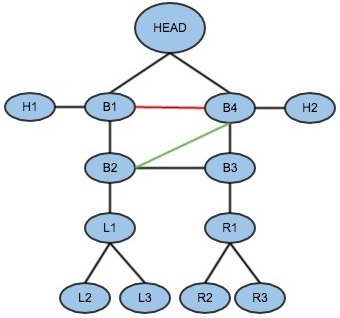
\includegraphics[width=0.75\linewidth]{figures/ml5.jpg}
    \caption{Moralized/Triangulated graph}
    \vspace{4ex}
  \end{subfigure}%%
  \begin{subfigure}[b]{0.5\linewidth}
    \centering
    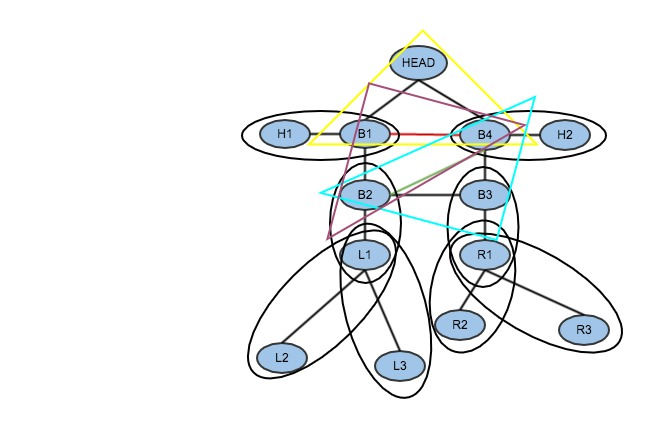
\includegraphics[width=0.75\linewidth]{figures/ml5triang.jpg}
    \caption{Clique graph}
    \vspace{4ex}
  \end{subfigure}
\end{figure}
\begin{figure}[ht]
    \centering
    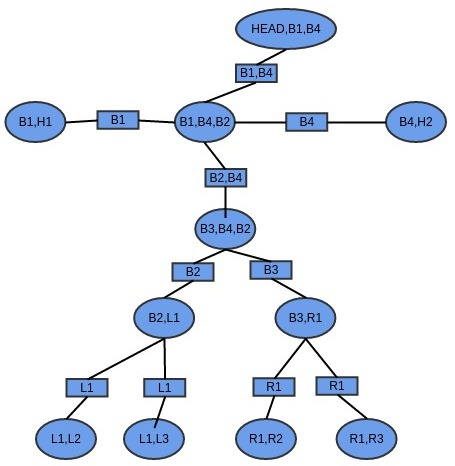
\includegraphics[width=0.5\textwidth]{figures/ml5JT.jpg}
    \caption{Junction Tree}
\end{figure}

\section*{4}

\section*{5}


\end{document}

